\documentclass[11pt]{article}

% ============================================================================
%  DRAFT arXiv paper, generated from thesis/cpad/writeup.md (Part 2).
%  refs.bib validated 2026-11-19 against the primary PDFs (titles/authors/venues OK;
%    santato2026, liu2025, ogilvie2025 titles corrected to match the sources).
%  REMAINING before any submission:
%   - set \artifacturl above to the pushed repo URL, then recompile
%   - author / affiliation / co-authorship left as-is per author's instruction
%   - responsible-disclosure statement intentionally omitted for now
% ============================================================================

\usepackage[utf8]{inputenc}
\usepackage[T1]{fontenc}
\usepackage{lmodern}
\usepackage[margin=1in]{geometry}
\usepackage{amsmath,amssymb,amsthm}
\usepackage{booktabs}
\usepackage{graphicx}
\usepackage{microtype}
\usepackage{xcolor}
\usepackage[numbers,sort&compress]{natbib}
\usepackage[colorlinks=true,linkcolor=blue!55!black,citecolor=blue!55!black,urlcolor=blue!55!black]{hyperref}
\usepackage{url}

\newtheorem{proposition}{Proposition}

\newcommand{\inner}[2]{\langle #1,\, #2\rangle}
\newcommand{\fto}{\texorpdfstring{FHEW$\to$CKKS}{FHEW-to-CKKS}}
\newcommand{\ctf}{\texorpdfstring{CKKS$\to$FHEW}{CKKS-to-FHEW}}
\newcommand{\Z}{\mathbb{Z}}
\newcommand{\out}{\mathsf{out}}
\newcommand{\code}[1]{\texttt{#1}}
% TODO: set \artifacturl to the pushed repo URL, then recompile. This is the ONLY place to change.
\newcommand{\artifacturl}{https://github.com/almantare/fhew-to-ckks-indcpad}

\title{\bfseries Recovering the FHEW Secret Key from \fto{}\\ Scheme Switching under IND-CPA-D}

% TODO: confirm authors / affiliation / co-author before submission
\author{%
  Artemiy Altamare\\[2pt]
  \small HSE University, MIEM, Moscow\\
  \small \texttt{aaaltamare@edu.hse.ru}%
}
\date{\today}

\begin{document}
\maketitle

\begin{abstract}
\citeauthor{santato2026}~\cite{santato2026} show that converting a CKKS ciphertext to FHEW
lets an IND-CPA-D adversary bypass CKKS's noise-flooding countermeasure and recover the CKKS
secret key. They implement the attack against OpenFHE but test only the \ctf{} direction,
explicitly noting that OpenFHE switches ``in both directions; we focus only on the
CKKS-to-FHEW direction.'' We settle the other direction. OpenFHE's \fto{} conversion
homomorphically evaluates LWE decryption; we measure its transfer function to be
$\out = (p/2\pi)\sin(2\pi\,\varphi/q)$, so the CKKS plaintext it returns is the LWE message
\emph{plus the LWE error attenuated by the scaling factor}. The switch shrinks the error and
leaves it inside the target scheme's message space. That makes
the attack immediate in the IND-CPA-D game: request an encryption of zero, apply the switching
oracle, and query decryption. Inverting the sine recovers each ciphertext's error exactly,
which gives a linear equation in the LWE secret. Because one switch packs many LWE ciphertexts
into CKKS slots, one decryption query yields $512$ equations, and \textbf{three queries recover
the full $1305$-coordinate STD128 FHEW secret key} (verified end to end, $1536/1536$ errors
exact). The general statement is that scheme switching transports the \emph{source} scheme's
error into the \emph{target} scheme's plaintext, so a decryption oracle on the target recovers
the \emph{source} secret. This direction matters in practice because every deployed
countermeasure is designed around CKKS's error, while nothing protects the LWE error, since FHEW is
treated as an exact scheme. OpenFHE's own
noise flooding, pushed to the largest setting the library accepts, does \textbf{not} stop the
attack; flooding calibrated to a propagated noise tag, as in Algorithm~6 of
\cite{santato2026}, does.
\end{abstract}

\section{Introduction}

Fully homomorphic encryption (FHE) libraries increasingly support \emph{scheme switching}:
converting a ciphertext of one FHE scheme into a ciphertext of another so that each scheme is
used where it is strongest --- CKKS~\cite{cheon2017} for SIMD real arithmetic, FHEW/TFHE~\cite{ducas2015}
for fast Boolean gates and comparisons. OpenFHE~\cite{openfhe} ships this feature for CKKS and FHEW in
both directions.

CKKS is an \emph{approximate} scheme: decryption returns the message plus a small error.
\citeauthor{limicciancio2021}~\cite{limicciancio2021} showed that this makes textbook CKKS
insecure under IND-CPA-D (indistinguishability under chosen-plaintext attack with a decryption
oracle), because the returned error is a linear function of the secret key. The standard
countermeasure is \emph{noise flooding}: before returning the decrypted value, add random noise
large enough to drown the secret-dependent error but small enough to preserve the intended
precision.

\citeauthor{santato2026}~\cite{santato2026} observe that scheme switching opens a new hole. To
recover the CKKS key they (i)~amplify the CKKS error by repeated doubling until it overflows into
the message space, (ii)~switch to FHEW --- an \emph{exact} scheme whose decryption applies no
flooding --- and (iii)~read the amplified error exactly from the FHEW decryption. Repeating over
many ciphertexts yields enough linear equations to solve for the CKKS secret.

Their proof-of-concept and analysis cover only \ctf{}. The \fto{} direction differs
in a way that makes the forward attack inapplicable --- the \emph{target} scheme is now CKKS, the
very scheme that floods --- and they leave it untested. This work analyzes and breaks that
direction.

\paragraph{Contributions.}
\begin{itemize}
  \item \textbf{C1.} We measure what OpenFHE's \fto{} actually computes. Its transfer function is
    $\out = (p/2\pi)\sin(2\pi\,\varphi/q)$, so the CKKS plaintext it returns is $m + e/\Delta$: the
    switch attenuates the LWE error and places it in the target scheme's message space
    (\S\ref{sec:computes}).
  \item \textbf{C2.} We give an IND-CPA-D key-recovery attack on \fto{} that uses only
    oracle-produced state entries --- request an encryption of zero, optionally scale it by a
    plaintext constant, switch, decrypt --- and reads each ciphertext's LWE error by inverting the
    sine (\S\ref{sec:attack}).
  \item \textbf{C3.} We implement it against OpenFHE (commit \code{ed361af2}) and recover a full
    STD128 FHEW secret key, $1305/1305$ coordinates, from \textbf{three decryption queries}, both
    at high precision and at the scaling modulus of the library's own example (\S\ref{sec:results}).
  \item \textbf{C4.} We delimit when flooding stops the attack (\S\ref{sec:flooding}). Flooding of
    \emph{fixed} magnitude is defeated by amplification; flooding calibrated to the ciphertext's
    propagated noise tag --- the construction of Algorithm~6 of~\cite{santato2026} --- scales with
    the amplification and defeats the attack at every factor we tested. We report this as a
    negative result against our own attack, and the lattice fallback also fails: the residual
    instance left by inexact error recovery is estimated at $2^{168}$ and above.
  \item \textbf{C5.} We report, and verify, that OpenFHE's switching key is itself a CKKS
    encryption of the FHEW secret exposed through a public accessor, so any deployment that
    decrypts an arbitrary well-formed ciphertext leaks the key in one query. We state the boundary
    between that and the in-game attack (\S\ref{sec:discussion}).
  \item \textbf{C6.} The algebraic core of the recovery --- that a solution of the collected
    system \emph{is} the secret, and that mod-2 pivot selection is sound over $\Z_{2^k}$ --- is
    machine-checked in Lean~4 with no \code{sorry}.
\end{itemize}

\section{Background}

\subsection{The schemes at a glance}
\label{sec:glance}

\paragraph{The common foundation: LWE and RLWE.}
Essentially all of today's FHE rests on the \emph{Learning With Errors} (LWE) problem and its ring
variant RLWE. An LWE sample hides a secret vector $s$ inside a noisy linear equation: from many
pairs $(a,\ \inner{a}{s} + e)$ with public random $a$ and a small random error $e$, recovering $s$
is believed hard. Encryption buries a message in such an equation; decryption, which knows $s$,
subtracts $\inner{a}{s}$ and is left with the message plus the small error $e$. \emph{RLWE} is the
same idea with the vectors replaced by polynomials in a ring $\Z_q[x]/(x^N+1)$, which lets a single
ciphertext carry many values at once and is what makes FHE practical. The error $e$ is the source of this hardness. This paper concerns what happens when a scheme lets an adversary read that error back.

\paragraph{FHEW: exact, bit-level.}
FHEW~\cite{ducas2015} (and its close relative TFHE) is an \emph{LWE}-based scheme specialised for
fast Boolean and small-integer operations, with a bootstrapping step that refreshes noise in
milliseconds. Its defining property for us is that it is \emph{exact}: decryption rounds the
recovered phase to the nearest message and returns that message, with no residual error.

\paragraph{CKKS: approximate, SIMD arithmetic.}
CKKS~\cite{cheon2017} is an \emph{RLWE}-based scheme for approximate arithmetic on vectors of real
or complex numbers --- a common choice for machine-learning workloads. Its defining
property is that it is \emph{approximate}. Decryption returns the message \emph{plus} the small
error, since for real-valued data a tiny perturbation is harmless. But that returned error is a
linear function of the secret key, so once a decryption result is shown to an adversary CKKS needs
a dedicated countermeasure (noise flooding, below).

\paragraph{Scheme switching.}
No single scheme is good at everything: CKKS multiplies vectors of reals cheaply but cannot compare
or branch; FHEW evaluates comparisons and table lookups but is clumsy at bulk arithmetic.
\emph{Scheme switching} converts a ciphertext of one into a ciphertext of the other, in place, so a
program can use each where it is strongest. OpenFHE~\cite{openfhe} ships switching between CKKS and
FHEW in both directions. The conversion is itself a homomorphic computation, carried out under a
public \emph{switching key}, which is an encryption of
one scheme's secret key under the other.

\paragraph{Noise flooding.}
Because CKKS decryption exposes a secret-dependent error, the standard fix is to add extra random
noise to the decrypted value before releasing it --- enough to statistically drown the
secret-dependent part, little enough to preserve the precision the user asked for. This
``flooding'' is the countermeasure every attack in this area must overcome. The forward attack of
\citeauthor{santato2026} avoids it by leaving CKKS. In the reverse direction, the flooding OpenFHE
ships does not stop our attack (\S\ref{sec:flooding}).

\subsection{LWE / FHEW}
An LWE ciphertext under secret $s \in \Z_q^n$ encrypting $m \in \Z_p$ is a pair $(a, b)$ with
$a \in \Z_q^n$ uniform and
\[
  b = \inner{a}{s} + \Delta m + e \pmod q, \qquad \Delta = \lfloor q/p \rfloor,
\]
where $e$ is a small error. Decryption computes the \emph{phase}
$\varphi = b - \inner{a}{s} = \Delta m + e \pmod q$ and rounds:
$m = \mathrm{round}(p\varphi/q) \bmod p$, correct when $|e| < \Delta/2$. OpenFHE's \code{binfhe}
follows exactly this convention. FHEW is \emph{exact}: decryption returns $m$ with no residual
error and no flooding.

\subsection{CKKS and noise flooding}
CKKS encrypts a vector $z \in \mathbb{C}^{N/2}$ as an RLWE ciphertext; decryption returns $z$ plus
a small error. The IND-CPA-D countermeasure (OpenFHE's \code{NOISE\_FLOODING\_DECRYPT}) adds
statistical noise $\nu$ to the decrypted value, calibrated to hide the secret-dependent error
while preserving a target precision. Flooding therefore lives in \emph{message space} and must
stay well below the message resolution or it corrupts the result.

\subsection{IND-CPA-D}
The adversary drives three stateful oracles (Definition~5 of~\cite{santato2026}, reproduced in
\S\ref{sec:attack}). $E(m_0, m_1)$ encrypts and records the pair of labels with the ciphertext in
a state $S$; $H(g, J)$ evaluates an admissible circuit on existing entries and records the images
of the labels; $D(i)$ decrypts the entry at index $i$, and answers only when that entry's two
labels agree. Against an approximate scheme the answer differs from the label, and that difference
is the leak the game measures. Two consequences matter here: the adversary cannot submit a
ciphertext of its own choosing to $D$ --- only an index --- and every circuit it applies must be a
function on the plaintext space, so that the challenger can track the labels.

\subsection{The forward attack (\ctf{}), recalled}
Start from a CKKS encryption of $0$ with RLWE error $e$; double it $k$ times so
$\|2^k e\|_\infty > \Delta/2$, so the error overflows into the message space; switch to FHEW; query
the (unflooded, exact) FHEW decryption to read $2^k e$; recover the CKKS key from
$e = b - a\cdot \mathit{sk}$ over many ciphertexts. The admissible amplification window has width
$W = \log p - \log\|e\|_\infty - \log\log n$.

\section{What \fto{} computes}
\label{sec:computes}

OpenFHE's \code{EvalFHEWtoCKKS} takes LWE ciphertexts and returns a CKKS ciphertext of their
\emph{messages}. Internally it homomorphically evaluates LWE decryption:
\begin{enumerate}
  \item It forms the public matrix $A$ (rows $a_i$) and vector $b$ from the input LWE ciphertexts.
  \item A \emph{switching key} --- a CKKS encryption of the LWE secret $s$ --- is used by
    \code{EvalPartialHomDecryption} to compute $A\cdot s$ under CKKS.
  \item It forms $b - A\cdot s = \Delta m + e \pmod q$: the LWE phase, encrypted under CKKS.
  \item A Chebyshev sine approximation followed by three double-angle steps evaluates the modular
    reduction, and the result is rescaled by $p$.
\end{enumerate}

\paragraph{What the output actually is.}
We measured it. Encrypting $m = 0..7$ and switching ($p = 256$) yields
decrypted slots $0.000, 0.9999, 1.9992, 2.9973, 3.9936, 4.9875, 5.9783, 6.9656$. These differ from
$m$ by more than approximation error: the Chebyshev sine plus three double-angle
steps, rescaled by $\code{postScale} = p$, computes
\[
  \out = \frac{p}{2\pi}\,\sin\!\left(\frac{2\pi\,\varphi}{q}\right), \qquad \varphi = \Delta m + e.
\]
That closed form reproduces all eight measured slots to five decimals. Expanding it for small
argument gives $\out \approx \varphi/\Delta = m + e/\Delta$: the switch transfers the phase and
attenuates the LWE error by
$\Delta$ (Figure~\ref{fig:transfer}). Legitimate users recover $m$ because $|e/\Delta| \ll \tfrac12$ and
they round. An adversary inverts the sine and recovers $e$.

\begin{figure}[t]
  \centering
  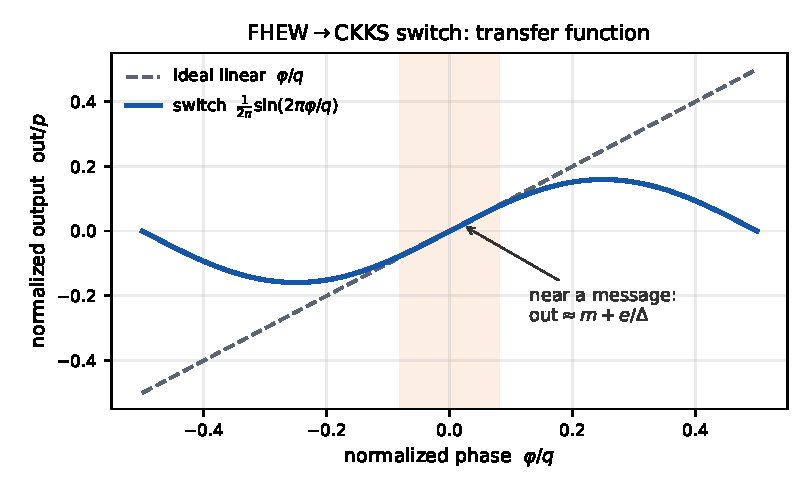
\includegraphics[width=0.62\linewidth]{fig_transfer.pdf}
  \caption{The \fto{} switch applies a sine transfer function to the LWE phase rather than
  rounding it. Near a message (shaded) the output is $m + e/\Delta$, so the LWE error survives,
  attenuated, inside CKKS message space and is recovered by inverting the sine.}
  \label{fig:transfer}
\end{figure}

\paragraph{Consequence for the countermeasure.}
The leaked quantity $e/\Delta$ is a \emph{sub-unit fraction} of a message unit, which is the
regime that noise flooding is designed to cover. Whether flooding
stops this attack is a quantitative question, settled in \S\ref{sec:flooding}.

\section{The attack}
\label{sec:attack}

\paragraph{The model.}
We work in the IND-CPA-D game as~\cite{santato2026} state it (their Definition~5, extended to
pipelines in Definition~11). The adversary drives three stateful oracles. $E(m_0, m_1)$ encrypts
and records $(m_0, m_1, ct)$ in the state. $H(g, J)$ evaluates an admissible circuit $g$ on
existing state entries and records the labels $g(m_0\dots)$, $g(m_1\dots)$. The switching oracle
$\mathit{SW}$ moves an entry from the source state to the target state, applying the plaintext map
$\tau$. Decryption is
\[
  D(i):\quad \text{if } S[i].m_0 = S[i].m_1 \ \text{ then return } \mathrm{Dec}(\mathit{sk}, S[i].ct)
  \ \text{ else return } \bot
\]
--- note that $D$ takes an \textbf{index into the state}, not a ciphertext supplied by the
adversary. This is used twice below.

\paragraph{The attack.}
Three oracle calls:
\begin{enumerate}
  \item $E(0, 0)$ --- a fresh FHEW encryption of zero enters the state with labels $m_0 = m_1 = 0$.
  \item $\mathit{SW}$ --- the entry moves to the CKKS state with label $\tau(0) = 0$.
  \item $D(i)$ --- the labels agree, so the oracle answers. The ideal plaintext is $0$. The actual
    decryption is $e/\Delta$.
\end{enumerate}
That difference is the IND-CPA-D leak. From \S\ref{sec:computes} the
switch's transfer function is $\out = (p/2\pi)\sin(2\pi\,\varphi/q)$, so
\[
  e = \frac{q}{2\pi}\,\arcsin\!\left(\out \cdot \frac{2\pi}{p}\right),
\]
recovered exactly by rounding. With the error in hand, $\inner{a}{s} = b - e \pmod q$ for the
public $(a, b)$, one linear equation per ciphertext.

At the scaling modulus used by OpenFHE's own example (50 bits) the CKKS evaluation noise swamps
$e/\Delta$ and this bare form fails (single digits out of $512$ exact across runs). One extra
oracle call fixes it: apply $H$ with $g(m) = t\cdot m \bmod p$ to the FHEW entry before switching.
This is a plaintext function --- the challenger records $g(0) = 0$ --- and it scales the
phase to $t\cdot e$, lifting the signal by a factor of $t$ while the CKKS noise is unchanged,
because $a$ is scaled modulo $q$ and stays uniform. At $t = 256$ the default configuration already
gives $512/512$.

The amplification serves only to measure the error: the linear equation must be
written with the \textbf{original} $(a, b)$. Using the scaled pair would both mis-scale the error
term and, for $t$ a power of two, make the coefficient matrix singular modulo $2$, which destroys
the pivot selection in the solve.

\paragraph{Efficiency.}
A single \code{EvalFHEWtoCKKS} packs up to \code{slots} LWE ciphertexts into the CKKS slots, and
one decryption returns all of them. One query therefore yields \code{slots} equations.

\subsection{The reduction}
We state the attack as a distinguisher so that the win condition is explicit.

\begin{proposition}
Let $\Pi$ be the OpenFHE \fto{} pipeline at the parameters of \S\ref{sec:results}, and let
\code{slots} be the CKKS slot count. There is an adversary $\mathcal{A}$ making
$q = \lceil n/\code{slots}\rceil$ decryption queries (three at our parameters) with advantage
$1/2 - \varepsilon$ in the $q$-IND-CPA-D game for $\Pi$, where $\varepsilon$ is the probability
that some recovered error is wrong or that no $n$ of the collected equations form a matrix
invertible modulo $2$.
\end{proposition}

\begin{proof}
$\mathcal{A}$ proceeds in two phases.

\emph{Phase 1 --- extraction.} Repeat for $j = 1 \dots q$: call $E(0, 0)$ \code{slots} times,
obtaining state entries whose label pairs are all $(0, 0)$, and record the public $(a_i, b_i)$ of
each returned ciphertext. Optionally call $H(g_t, \cdot)$ on each entry with
$g_t(m) = t\cdot m \bmod p$; the challenger records $g_t(0) = 0$ on both sides, so the labels still
agree. Call $\mathit{SW}$ on the vector of those entries; it produces one target entry, with label
$\tau(0, \dots, 0) = (0, \dots, 0)$. Call $D$ on that index: the two labels agree, so the oracle
answers. Slot $i$ of the answer is
\[
  \out_i = \frac{p}{2\pi}\,\sin\!\left(\frac{2\pi\,t\,e_i}{q}\right) + \eta_i,
\]
with $\eta_i$ the CKKS evaluation error. $\mathcal{A}$ sets
$\hat{e}_i = \mathrm{round}\!\big(\tfrac{q}{2\pi t}\arcsin(\out_i \cdot 2\pi/p)\big)$ and records the
equation $\inner{a_i}{s} = b_i - \hat{e}_i \pmod q$ --- written with the \textbf{original}
$(a_i, b_i)$, not the scaled pair.

\emph{Phase 2 --- decision.} $\mathcal{A}$ selects $n$ equations whose matrix $A$ is invertible
modulo $2$ and solves $A x = v \pmod q$ by Hensel lifting. If every $\hat{e}_i$ equals $e_i$, then
$x = s$: this is exactly the uniqueness statement machine-checked in
\code{lean/LWEKeyRecovery.lean} (\code{secret\_unique}, \code{key\_recovery}, and
\code{isUnit\_det\_iff\_map\_two} for the mod-2 selection). $\mathcal{A}$ then calls $E(m_0, m_1)$
with $m_0 \neq m_1$, obtaining a challenge ciphertext $(a^*, b^*)$; it may not query $D$ on it,
because the labels differ --- but it no longer needs to. $\mathcal{A}$ computes
$m = \mathrm{round}(p\,(b^* - \inner{a^*}{s})/q)$ itself and outputs $0$ if $m = m_0$, else $1$.

$\mathcal{A}$ is correct whenever extraction succeeded and LWE decryption is correct on the
challenge, so its advantage is $1/2 - \varepsilon$.
\end{proof}

\paragraph{On $\varepsilon$.}
Across $1536$ collected equations every recovered error was
exact (\S\ref{sec:results}), and the selected matrix had full rank $1305$ over $\mathrm{GF}(2)$. A
single wrong error is fatal --- the solve then returns a vector with no
coordinate in $\{-1,0,1\}$. Our evidence supports
a rule-of-three bound on $\varepsilon$: $0$ failures in $1536$ gives per-equation exactness
$\geq 99.8\%$ at $95\%$ confidence.

\paragraph{What the reduction needs, and what it does not.}
It needs only $E$, $H$ with a plaintext function, $\mathit{SW}$, and $D$ on an index whose labels
agree. It submits no ciphertext of its own construction to $D$, so it is admissible, whereas both the
switching-key query of \S\ref{sec:discussion} and our own
earlier boundary probe are not.

\paragraph{Solving.}
The equations $\inner{a_j}{s} = v_j \pmod q$ with exact $v_j$ and ternary $s$ are solved directly.
Since $q = 2^{28}$ is a prime power, any $n$ equations whose matrix is invertible modulo $2$ have
unit determinant modulo $q$; we select them with one Gauss step over $\mathrm{GF}(2)$ and
Hensel-lift the solution from mod $2$ to mod $2^{28}$. The algebraic core of this step --- including
the claim that a solution of the collected system \emph{is} the secret, so the adversary needs no
ground truth to know it succeeded --- is machine-checked in Lean (\code{lean/LWEKeyRecovery.lean}).

\section{Implementation and results}
\label{sec:results}

PoC against OpenFHE commit \code{ed361af2}.\footnote{Artifact (C\texttt{++} proof-of-concept,
Lean~4 proof, and the result logs cited here): \url{\artifacturl}.} CKKS: ring dimension $2^{13}$, multiplicative depth
$13$, FIXEDAUTO rescaling, scaling modulus $59$ bits. FHEW: STD128, $\log q = 28$, LWE dimension
$n = 1305$, $q = 2^{28}$; LWE plaintext modulus $p = 256$, $\Delta = 2^{20}$. \code{poc/direct.cpp},
$512$ slots.

\begin{table}[h]
\centering
\begin{tabular}{lr}
\toprule
quantity & value \\
\midrule
equations per decryption query & $512$ \\
decryption queries for the whole key ($n = 1305$) & \textbf{3} \\
errors recovered exactly & \textbf{$1536 / 1536$} \\
RMS / max error of the recovered $e$ & $0.0104 / 0.0340$ \\
key recovery & \textbf{$1305 / 1305$ coordinates}, $14.8$\,s \\
\bottomrule
\end{tabular}
\end{table}

At OpenFHE's own example setting (scaling modulus $50$) with the amplification step at $t = 1024$:
$1536/1536$ errors exact (RMS $0.016$), and again \textbf{$1305/1305$ coordinates} recovered from
\textbf{three decryption queries}. The break therefore covers the library's example configuration.

The solve also reports that all $1536$ collected equations are satisfied by the recovered vector, a
check that uses no ground truth --- by the uniqueness theorem the adversary knows it has the key.

An earlier version of this work located the error by sweeping a shift of $b$ across the message
period and fitting the resulting ramp. That version needed roughly $350$ switch calls and a
calibration probe, reached only $0.13$ maximum error, and was \textbf{not
admissible}: shifting $b$ by a constant that is not a multiple of $\Delta$ is not a function on the
FHEW plaintext space, so $H$ cannot perform it and the challenger has no label for the result. The
direct read replaces it.

\section{Flooding: what the library does, and what would be needed}
\label{sec:flooding}

\paragraph{(a) OpenFHE's own countermeasure, actually enabled, does not stop the attack.}
Setting \code{NOISE\_FLOODING\_DECRYPT} with \code{EXEC\_EVALUATION} and a noise estimate is the
protection a user can switch on today. The library caps how far it may be pushed: context
generation refuses with \emph{``Precision of less than 3 bits is not supported. logstd $16.79$ +
noiseEstimate $40.0$ must be $56$ or less''}, so at these parameters the estimate cannot exceed
$\approx 39.2$. Sweeping it up to that ceiling:

\begin{table}[h]
\centering
\begin{tabular}{lcccccccc}
\toprule
noise estimate & $10$ & $20$ & $28$ & $32$ & $35$ & $38$ & $39$ & $40$ \\
\midrule
errors exact (of $512$) & $512$ & $512$ & $512$ & $512$ & $512$ & $512$ & $\mathbf{512}$ & refused \\
\bottomrule
\end{tabular}
\end{table}

At every admissible setting, including the largest one the library will build, all $512$ errors are
still recovered exactly (RMS $0.010$--$0.015$). The shipped countermeasure is calibrated to hide
the CKKS error; the quantity we read is a message-space value of size $e/\Delta$, and it survives.

\paragraph{(b) Synthetic flooding of fixed magnitude is defeated by amplification.}
Injecting Gaussian noise of standard deviation $\sigma$ directly into each decrypted slot, the bare
read fails once $\sigma$ exceeds about $4$ phase units ($\sigma = 1024$ gives $0/40$). Scaling the
LWE ciphertext by $t$ before switching restores it, because the signal grows by $t$ while the
injected noise does not: $0 \to 10 \to 40$ out of $40$ as $t$ goes $1 \to 64 \to 1024$.

\paragraph{(c) Flooding calibrated to a propagated noise tag would stop it.}
In Algorithm~6 of~\cite{santato2026} each ciphertext carries a noise tag updated at every
homomorphic operation, and decryption floods relative to that tag. Our amplification is a scalar
multiplication, so it multiplies the tag as well. Re-running with $\sigma$ scaled proportionally to
$t$:

\begin{table}[h]
\centering
\begin{tabular}{lccc}
\toprule
$t$ & $1$ & $64$ & $1024$ \\
\midrule
exact, fixed $\sigma$     & $0/40$ & $10/40$ & $40/40$ \\
exact, $\sigma \propto t$ & $0/40$ & $0/40$  & $0/40$ \\
\bottomrule
\end{tabular}
\end{table}

Amplification then gains nothing, as the authors anticipate: of their own $2^k$
amplification they write that a switch with good ciphertext hygiene ``would instead hide from us
the new ciphertexts adaptively on $k$''.

\paragraph{The gap between (a) and (c).}
The defence specified in~\cite{santato2026} works. The defence that ships in
OpenFHE is weaker and cannot be configured up to the required strength ---
the library refuses beyond $\approx 39.2$, and the tag-scaled magnitude needed to cover an
amplified query is far above that. There is also no fallback for the adversary when the leak
\emph{is} covered: the residual instance left by inexact error recovery is an LWE problem with
$n = 1305$, $q = 2^{28}$ and error $\sigma \geq 12.6$, which the stock Lattice
Estimator~\cite{latticeestimator} puts at $2^{168}$ and above ($2^{191}$ and $2^{216}$ at the
flooded settings). Below the exactness threshold the attack fails outright.

\section{Discussion}
\label{sec:discussion}

\paragraph{The switching key objection.}
OpenFHE's \code{EvalFHEWtoCKKSKeyGen} sets the switching key to a CKKS encryption of the FHEW
secret --- the source comment says exactly that --- and exposes it through the public accessor
\code{cc->GetSwkFC()}. Decrypting it returns all $1305$ coordinates at once; we verified this
(\code{poc/swktest.cpp}, max error $2\mathrm{e}{-13}$). Two consequences follow.

First, inside the game this query is inadmissible: $D$ takes a state index and the switching key is
never a state entry, so an adversary restricted to the oracles cannot make it. Our attack uses only
state entries and is therefore an IND-CPA-D break; the trivial one is not available in that
model.

Second, outside the game the trivial break dominates. Any deployment whose decryption service
accepts an arbitrary well-formed CKKS ciphertext hands over the FHEW key in one query, because the
switching key \emph{is} such a ciphertext. In practice, neither the switching key nor a
decryption oracle on switched ciphertexts should be exposed, since three queries suffice against the latter.

\paragraph{How much is new?}
A pipeline ending in a vanilla
CKKS decryption has been known to be IND-CPA-D-insecure since Li and Micciancio. What is specific
here is the target: the oracle is on CKKS, but what falls is the \textbf{FHEW} secret. The forward
attack had to amplify to move CKKS error into FHEW's message space; here the switch delivers the
LWE error into CKKS's message space directly.

\paragraph{Remedies.}
Flooding calibrated to a propagated noise tag, as in Algorithm~6
of~\cite{santato2026}, covers the leak (\S\ref{sec:flooding}), and ciphertext hygiene would
refuse to return the component at all. OpenFHE implements neither; fixed-magnitude flooding is
defeated by amplification.

\paragraph{Related work, and why it does not overlap.}
Two recent lines sit closest. \citeauthor{liu2025}~\cite{liu2025} attack the IND-CPA-D security of
\emph{relaxed functional bootstrapping} in the FHEW/TFHE family; their lever is bootstrapping
failure probability, and the mitigation is to drive that probability
negligible. \citeauthor{ogilvie2025}~\cite{ogilvie2025} goes the other way and builds provable
IND-CPA-D and KR-D security for approximate HE with substantially less decryption noise than earlier
provable constructions, partly by treating rescale noise as a HintLWE hint. That work is the
constructive counterpart to our \S\ref{sec:flooding}: it shows that a low-overhead
flooding with provable guarantees exists, and OpenFHE ships a different one. Neither
paper addresses the switching direction studied here; a search of the ePrint corpus for
scheme-switching security returns only~\cite{santato2026}.

\section{Conclusion}

The \fto{} direction of OpenFHE scheme switching is IND-CPA-D-insecure, and cheaply so: three
decryption queries recover a full STD128 FHEW secret key, using only oracle-produced state entries.
The switch leaks because it outputs $m + e/\Delta$, so the source
scheme's error lands in the target scheme's plaintext. Separately, the switching key is a
decryptable encryption of that same secret, which breaks any deployment that will decrypt an
arbitrary ciphertext. The defence proposed in~\cite{santato2026} --- ciphertext hygiene with
flooding calibrated to a propagated noise tag --- appears to close the first hole, and our
measurements support that; the second is closed by not publishing the key. Neither is implemented
in what users get today.

\bibliographystyle{plainnat}
\bibliography{refs}

\end{document}
